% This file provides a template to format JASSS articles v.0.5, 2015-03-24

% In order to be compiled, the following packages should be installed in your system:
% graphicx,xcolor, booktabs,amsmath, ifthen, geometry, authblk, natbib, endnotes
 
 % Please use pdflatex

% The font used is Source Sans Pro, normally included in Tex Live and other  major LaTeX distributions
% Location at CTAN: http://www.ctan.org/tex-archive/fonts/sourcesanspro/
% See also: http://www.tug.dk/FontCatalogue/sourcesanspro/

%%%%%%%%%%%%%%%%%%%%%%%%%%%%%%%%%%%%%%%%%%%%%%

\documentclass{JASSS}
	
%%%%%%%%%%%%%%%%%%%%%%%%%%%%%%%%%%%%%%%%%%%%%%

% Editorial fields (to be set in case of publication)	
% Please leave this section untouched
%\doinum{10.18564/jasss.xxxx}
%\volume{xx}
%\issue{x}
%\article{x}
%\pubyear{20xx}
%\received{dd-mmm-yyyy}
%\accepted{dd-mmm-yyyy}
%\published{dd-mmm-yyyy}

%%%%%%%%%%%%%%%%%%%%%%%%%%%%%%%%%%%%%%%%%%%%%% 

% title, authors and affiliations	

\title{The Agent's new Cloths \\ {\large Towards functional programming in Agent-Based Simulation}}

%All authors should be included in the submission. To anonymise the submission, set to 'true' the \reviewcopy command below. However, before submitting  you can check that all the informations you entered are correct by temporarily setting it to 'false'. Please remember to set it back to 'true' before the submission.
\reviewcopy{true} 

\author[1]{Jonathan Thaler}
\author[1]{Peer-Olaf Siebers}
\author[1]{Thorsten Altenkirch}
\affil[1]{University of Nottingham, 7301 Wollaton Rd, Nottingham, NG8 1BB, United Kingdom}

% Subsequent author should be included using the following template. You can add more in case of need, just remember to appropriately set the corresponding number.  Please check the the authblk package documentation  in case of doubts

%\author[2]{Second author here}
%\affil[2]{Affiliation of the second author here}

%\author[3]{Third author here}
%\affil[3]{Affiliation of the third author here}

%\author[4]{fourth author here}
%\affil[4]{fourth of the third author here}

% In case of multiple affiliation for the same author:

%\author[1,2]{Author name here}
%\affil[1]{First affiliation}
%\affil[2]{Second affiliation}

%  In case of several authors sharing the same affiliation:

%\author[1]{First author name}
%\author[1]{Second author name}
%\affil[1]{Affiliation}

% email for the corresponding author
\email{jonathan.thaler@nottingham.ac.uk}

%%%%%%%%%%%%%%%%%%%%%%%%%%%%%%%%%%%%%%%%%%%%%%

% NOTES. Please use endnotes. Notes should be placed after the main text and appendices and before the references. Also remember to uncomment the \theendnotes commands at the end of the document (just before the references)

%%%%%%%%%%%%%%%%%%%%%%%%%%%%%%%%%%%%%%%%%%%%%%

% REFERENCES should be included using the \citep, \citet, etc. commands provided by the natbib package

\usepackage{natbib}
	\setcitestyle{authoryear,round,aysep={}}
	
%%%%%%%%%%%%%%%%%%%%%%%%%%%%%%%%%%%%%%%%%%%%%%	

% EXTRA PACKAGES. Please place here any extra package you need along with your own command definitions
%\usepackage{graphicx}
%\usepackage{xcolor}
%\usepackage{booktabs}
%\usepackage{amsmath}
%\usepackage{ifthen}
%\usepackage{geometry}
%\usepackage{authblk}
%\usepackage{natbib}
%\usepackage{endnotes}
%\usepackage{minted}
\usepackage{hyperref}

%%%%%%%%%%%%%%%%%%%%%%%%%%%%%%%%%%%%%%%%%%%%%%

\begin{document}
\maketitle 

%%%%%%%%%%%%%%%%%%%%%%%%%%%%%%%%%%%%%%%%%%%%%%

% Abstract and keywords

\begin{abstract}
TODO: parallelism for free because all isolated e.g. running multiple replications or parameter-variations

TODO: it is paramount not to write against the established approach but for the functional approach. not to try to come up with arguments AGAINST the object-oriented approach but IN FAVOUR for the functional approach. In the end: dont tell the people that what they do sucks and that i am the saviour with my new method but: that i have a new method which might be of interest as it has a few nice advantages.

So far, the pure functional paradigm hasn't got much attention in Agent-Based Simulation (ABS) where the dominant programming paradigm is object-orientation, with Java, Python and C++ being its most prominent representatives. We claim that functional programming using Haskell is very well suited to implement complex, real-world agent-based models and brings with it a number of benefits. In this paper we will introduce the reader to the functional programming paradigm and explain how it can be applied to implementing ABS. Further we discuss benefits and advantages. As use-case we implemented the seminal Sugarscape model in Haskell.
\end{abstract}

\begin{keywords}
Agent-Based Simulation, Functional Programming, Haskell
\end{keywords}

%%%%%%%%%%%%%%%%%%%%%%%%%%%%%%%%%%%%%%%%%%%%%%
% Start of  paragraph numbering. Please leave this untouched
\parano{}

%%%%%%%%%%%%%%%%%%%%%%%%%%%%%%%%%%%%%%%%%%%%%%

% MAIN TEXT

\section{Introduction}
There exists a large number of simulation packages which allow the convenient creation of System Dynamics simulations by straight-forward visual diagram creation. One simply creates stocks and flows, connects them, specifies the flow-rates and initial parameters and then runs the model. An example for such a visual diagram creation in the simulation package AnyLogic can be seen in Figure \ref{fig:sir_stockflow_diagram}.

\begin{figure}
	\centering
	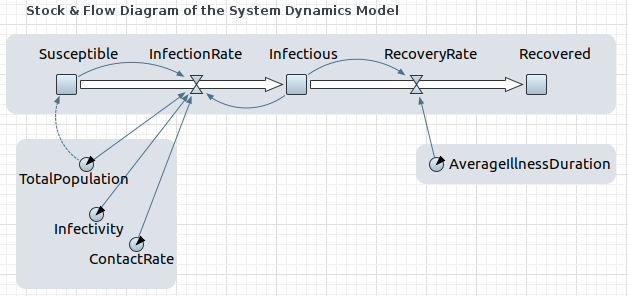
\includegraphics[width=.5\textwidth, angle=0]{./fig/SIR_SD_STOCKFLOW_DIAGRAMM.png}
	\caption{Visual System Dynamics Diagram of the SIR model in AnyLogic Personal Learning Edition 8.3.1.}
	\label{fig:sir_stockflow_diagram}
\end{figure}

Still, implementing System Dynamics directly in code is not as straight forward and involves numerical integration which can be quite tricky to get right. Thus, the aim of this paper is to look into how System Dynamics models can be implemented in code correctly without the use of a simulation package. We use the well known SIR model \cite{kermack_contribution_1927} from epidemiology to demonstrate our approach.

Our language of choice is Haskell because it emphasises a declarative programming style in which one describes \textit{what} instead of \textit{how} to compute. Further it allows to rule out interference with non-deterministic influences or side-effects already at compile-time. This is of fundamental importance for System Dynamics because it behaves completely deterministic and involves no stochastics or non-determinism whatsoever. Also, we make use of Functional Reactive Programming which allows to express continuous-time systems in a functional way. 

We show that by this approach we can arrive at correct-by-construction implementations of System Dynamic models. This means that the correctness of the code is obvious because we have closed the gap between the model specification and its implementation. Thus, the contribution of the paper is the demonstration of how to implement correct-by-construction System Dynamics simulations using Haskell and Functional Reactive Programming.

\section{Concepts of Functional Programming}
The reason why functional programming is called \textit{functional} is because because it makes functions the main concept of programming, promoting them to first-class citizens as we will describe later on. Its roots lie in the Lambda Calculus which was first described by Alonzo Church \citep{church_unsolvable_1936}. This is a fundamentally different approach to computation than imperative and object-oriented programming which roots lie in the Turing Machine \citep{turing_computable_1937}. Rather than describing \textit{how} something is computed as in the more operational approach of the Turing Machine, due to the more declarative nature of the Lambda Calculus, code in functional programming describes \textit{what} is computed.

In our research we are using the functional programming language Haskell. The paper of \citep{hudak_history_2007} gives a comprehensive overview over the history of the language, how it developed and its features and is very interesting to read and get accustomed to the background of the language. The main points why we decided to go for Haskell are:

\begin{itemize}
	\item Rich Feature-Set - it has all fundamental concepts of the pure functional programming paradigm of which we explain the most important below.
	\item Real-World applications - the strength of Haskell has been proven through a vast amount of highly diverse real-world applications \cite{hudak_history_2007}, is applicable to a number of real-world problems \cite{osullivan_real_2008} and has a large number of libraries available \footnote{\url{https://wiki.haskell.org/Applications_and_libraries}}.
	\item Modern - Haskell is constantly evolving through its community and adapting to keep up with the fast changing field of computer science. Further, the community is the main source of high-quality libraries.
\end{itemize}

As a short example we give an implementation of the factorial function in Haskell:
\begin{HaskellCode}
factorial :: Integer -> Integer
factorial 0 = 1
factorial n = n * factorial (n-1)
\end{HaskellCode}

When looking at this function we can already see the central concepts of functional programming: 
\begin{enumerate}
	\item Declarative - we describe \textit{what} the factorial function is rather than how to compute it. This is supported by \textit{pattern matching} which allows to give multiple equations for the same function, matching on its input. 
	\item Immutable data - in functional programming we don't have mutable variables - after a variable is assigned, it cannot change its contents. This also means that there is no destructive assignment operator which can re-assign values to a variable. To change values, we employ recursion.
	\item Recursion - the function calls itself with a smaller argument and will eventually reach the case of 0. Recursion is the very meat of functional programming because they are the only way to implement loops in this paradigm due to immutable data.
	\item Static Types - the first line indicates the name and the types of the function. In this case the function takes one Integer as input and returns an Integer as output. Types are static in Haskell which means that there can be no type-errors at run-time e.g. when one tries to cast one type into another because this is not supported by this kind of type-system.
	\item Explicit input and output - all data which are required and produced by the function have to be explicitly passed in and out of it. There exists no global mutable data whatsoever and data-flow is always explicit.
	\item Referential transparency - calling this function with the same argument will \textit{always} lead to the same result, meaning one can replace this function by its value. This means that when implementing this function one can not read from a file or open a connection to a server. This is also known as \textit{purity} and is indicated in Haskell in the types which means that it is also guaranteed by the compiler.
\end{enumerate}

It may seem that one runs into efficiency-problems in Haskell when using algorithms which are implemented in imperative languages through mutable data which allows in-place update of memory. The seminal work of \cite{okasaki_purely_1999} showed that when approaching this problem from a functional mind-set this does not necessarily be the case. The author presents functional data structures which are asymptotically as efficient as the best imperative implementations and discusses the estimation of the complexity of lazy programs.

For an excellent and widely used introduction to programming in Haskell we refer to \cite{hutton_programming_2016}. Other, more exhaustive books on learning Haskell are \cite{lipovaca_learn_2011, allen_haskell_2016}. For an introduction to programming with the Lambda-Calculus we refer to \cite{michaelson_introduction_2011}. For more general discussion of functional programming we refer to \cite{hughes_why_1989, maclennan_functional_1990, hudak_history_2007}.

\subsection{Lazy evaluation, Higher Order Functions and Currying}
TODO: 

\subsection{Side-Effects}
One of the fundamental strengths of functional programming and Haskell is their way of dealing with side-effects in functions. A function with side-effects has observable interactions with some state outside of its explicit scope. This means that the behaviour it depends on history and that it loses its referential transparency character, which makes understanding and debugging much harder. Examples for side-effects are (amongst others): modifying a global variable, await an input from the keyboard, read or write to a file, open a connection to a server, drawing random-numbers,...

Obviously, to write real-world programs which interact with the outside-world we need side-effects. Haskell allows to indicate in the \textit{type} of a function that it does or does \textit{not} have side-effects. Further there are a broad range of different effect types available, to restrict the possible effects a function can have to only the required type. This is then ensured by the compiler which means that a program in which one tries to e.g. read a file in a function which only allows drawing random-numbers will fail to compile. Haskell also provides mechanisms to combine multiple effects e.g. one can define a function which can draw random-numbers and modify some global data. The most common side-effect types are:
\begin{itemize}
	\item IO - Allows all kind of I/O related side-effects: reading/writing a file, creating threads, write to the standard output, read from the keyboard, opening network-connections, mutable references,... 
	\item Rand - Allows to draw random-numbers.
	\item Reader - Allows to read from an environment.
	\item Writer - Allows to write to an environment.
	\item State - Allows to read and write an environment.
\end{itemize}

A function with side-effects has to indicate this in their type e.g. if we want to give our factorial function for debugging purposes the ability to write to the standard output, we add IO to its type: factorial :: Integer -> IO Integer. A function without any side-effect type is called \textit{pure}. A function with a given effect-type needs to be executed with a given effect-runner which takes all necessary parameters depending on the effect and runs a given effectful function returning its return value and depending on the effect also an effect-related result. For example when running a function with a State-effect one needs to specify the initial environment which can be read and written. After running such a function with a State-effect the effect-runner returns the changed environment in addition with the return value of the function itself. Note that we cannot call functions of different effect-types from a function with another effect-type, which would violate the guarantees. Calling a \textit{pure} function though is always allowed because it has by definition no side-effects. An effect-runner itself is a \textit{pure} function. The exception to this is the IO effect type which does not have a runner but originates from the \textit{main} function which is always of type IO.

Although it might seem very restrictive at first, we get a number of benefits from making the type of effects we can use explicit. First we can restrict the side-effects a function can have to a very specific type which is guaranteed at compile time. This means we can have much stronger guarantees about our program and the absence of potential errors already at compile-time which implies that we don't need test them with e.g. unit-tests. Second, because effect-runners are themselves \textit{pure}, we can execute effectful functions in a very controlled way by making the effect-context explicit in the parameters to the effect-runner. This allows a much easier approach to isolated testing because the history of the system is made explicit.

For a technical, in-depth discussion of the concept of side-effects and how they are implemented in Haskell using Monads, we refer to the following papers: \cite{moggi_computational_1989, wadler_essence_1992, wadler_monads_1995, wadler_how_1997, jones_tackling_2002}.

\subsection{Parallelism and Concurrency}
TODO: write this section

Also Haskell makes a very clear distinction between parallelism and concurrency. Parallelism is always deterministic and thus pure without side-effects because although parallel code runs concurrently, it does by definition not interact with data of other threads. This can be indicated through types: we can run pure functions in parallel because for them it doesn't matter in which order they are executed, the result will always be the same due to the concept of referential transparency. Concurrency is potentially non-deterministic because of non-deterministic interactions of concurrently running threads through shared data. Although data in functional programming is immutable, Haskell provides primitives which allow to share immutable data between threads. Accessing these primitives is but only possible from within an IO or STM context which means that when we are using concurrency in our program, the types of our functions change from pure to either IO or STM effect context.

Spawning thousands of threads in Haskell is no problem and has very low memory footprint because they are lightweight user-space threads, managed by the Haskell Runtime System which maps them to physical operating-system threads. 

TODO: in haskell we can distinguish between parallelism and concurrency in the types: parallelism is pure, concurrency is impure
TODO: parallelism for free because all isolated e.g. running multiple replications or parameter-variations

TODO: For a technical, in-depth discussion on parallelism and concurrency in Haskell we refer to the excellent book \cite{marlow_parallel_2013}.

TODO: explain STM, Problem: live locks, For a technical, in-depth discussion on Software Transactional Memory in Haskell we refer to the following papers: \citep{harris_composable_2005, discolo_lock_2006, osullivan_real_2008, perfumo_limits_2008}. TODO: need much more papers on STM, parallelism and concurrency

\subsection{Functional Reactive Programming}
\label{sec:frp}
Functional Reactive Programming (FRP) is a way to implement systems with continuous and discrete time-semantics in functional programming. The central concept in FRP is the Signal Function which can be understood as a process over time which maps an input- to an output-signal. A signal in turn, can be understood as a value
which varies over time. Thus, signal functions have an awareness of the passing of time by having access to a $\Delta t$ which are positive time-steps with which the system is sampled. In general, signal functions can be understood to be computations that represent processes, which have an input of a specific type, process it and output a new type. Note that this is an important building block to represent agents in functional programming: by implementing agents as signal functions allows us to implement them as processes which act continuously over time, which implies a time-driven approach to ABS. We have also applied the concept of FRP to event-driven ABS \citep{meyer_event-driven_2014}.

FRP provides a number of functions for expressing time-semantics, generating events and making state-changes of the system. They allow to change system behaviour in case of events, run signal functions, generate deterministic (after fixed time) and stochastic (exponential arrival rate) events and provide random-number streams. 

TODO: libraries Yampa and Dunai

For a technical, in-depth discussion on FRP in Haskell we refer to the following papers: \citep{wan_functional_2000, hughes_generalising_2000, hughes_programming_2005, nilsson_functional_2002, hudak_arrows_2003, courtney_yampa_2003, perez_functional_2016, perez_extensible_2017}

\subsection{Property-Based Testing}
TODO: write this section

Although property-based testing has been brought to non-functional languages like Java and Python as well, it has its origins in Haskell and it is here where it truly shines.

We found property-based testing particularly well suited for ABS. Although it is now available in a wide range of programming languages and paradigms, propert-based testing has its origins in Haskell \citep{claessen_quickcheck:_2000, claessen_testing_2002} and we argue that for that reason it really shines in pure functional programming. Property-based testing allows to formulate \textit{functional specifications} in code which then the property-testing library (e.g. QuickCheck \citep{claessen_quickcheck:_2000}) tries to falsify by automatically generating random test-data covering as much cases as possible. When an input is found for which the property fails, the library then reduces it to the most simple one. It is clear to see that this kind of testing is especially suited to ABS, because we can formulate specifications, meaning we describe \textit{what} to test instead of \textit{how} to test (again the declarative nature of functional programming shines through). Also the deductive nature of falsification in property-based testing suits very well the constructive nature of ABS.

For a technical, in-depth discussion on property-based testing in Haskell we refer to the following papers: \citep{claessen_quickcheck:_2000, claessen_testing_2002}.

%\subsection{Software Transactional Memory}
%Although there exist STM implementations in non-functional languages like Java and Python, due to the nature of Haskells type-system, the use of STM has unique benefits in this setting.
%
%Concurrent programming is notoriously difficult to get right because reasoning about the interactions of multiple concurrently running threads and low level operational details of synchronisation primitives and locks is \textit{very hard}. The main problems are:
%
%\begin{itemize}
%	\item Race conditions due to forgotten locks.
%	\item Deadlocks resulting from inconsistent lock ordering.
%	\item Corruption caused by uncaught exceptions.
%	\item Lost wakeups induced by omitted notifications.
%\end{itemize}
%
%Worse, concurrency does not compose. It is utterly difficult to write two functions (or methods in an object) acting on concurrent data which can be composed into a larger concurrent behaviour. The reason for it is that one has to know about internal details of locking, which breaks encapsulation and makes composition depend on knowledge about their implementation. Also it is impossible to compose two functions e.g. where one withdraws some amount of money from an account and the other deposits this amount of money into a different account: one ends up with a temporary state where the money is in none of either accounts, creating an inconsistency - a potential source for errors because threads can be rescheduled at any time.
%
%STM promises to solve all these problems for a very low cost. In STM one executes actions atomically where modifications made in such an action are invisible to other threads until the action is performed. Also the thread in which this action is run, doesn't see changes made by other threads - thus execution of STM actions are isolated. When a transaction exists one of the following things will occur:
%
%\begin{enumerate}
%	\item If no other thread concurrently modified the same data as us, all of our modifications will simultaneously become visible to other threads.
%	\item Otherwise, our modifications are discarded without being performed, and our block of actions is automatically restarted.
%\end{enumerate}
%
%Note that the ability to \textit{restart} a block of actions without any visible effects is only possible due to the nature of Haskells type-system which allows being explicit about side-effects: by restricting the effects to STM only ensures that no uncontrolled effects, which cannot be rolled-back, occur.
%
%STM is implemented using optimistic synchronisation. This means that instead of locking access to shared data, each thread keeps a transaction log for each read and write to shared data it makes. When the transaction exists, this log is checked whether other threads have written to memory it has read - it checks whether it has a consistent view to the shared data or not. This might look like a serious overhead but the implementations are very mature by now, being very performant and the benefits outweigh its costs by far.
%
%Applying this to our agents is very simple: because we already use Dunai / BearRiver as our FRP library, we can run in arbitrary Monadic contexts. This allows us to simply run agents within an STM Monad and execute each agent in their own thread. This allows then the agents to communicate concurrently with each other using the STM primitives without problems of explicit concurrency, making the concurrent nature of an implementation very transparent. Further through optimistic synchronisation we should arrive at a much better performance than with low level locking.
%
%Problem: live locks
%
%For a technical, in-depth discussion on Software Transactional Memory in Haskell we refer to the following papers: \citep{harris_composable_2005, osullivan_real_2008}.

\section{Advanced Functional Programming Features}

\subsection{Functional Reactive Programming}
Functional Reactive Programming (FRP) is a way to implement systems with continuous and discrete time-semantics in functional programming. The central concept in FRP is the Signal Function which can be understood as a process over time which maps an input- to an output-signal. A signal in turn, can be understood as a value
which varies over time. Thus, signal functions have an awareness of the passing of time by having access to a $\Delta t$ which are positive time-steps with which the system is sampled. In general, signal functions can be understood to be computations that represent processes, which have an input of a specific type, process it and output a new type. Note that this is an important building block to represent agents in functional programming: by implementing agents as signal functions allows us to implement them as processes which act continuously over time, which implies a time-driven approach to ABS. We have also applied the concept of FRP to event-driven ABS \citep{meyer_event-driven_2014}.

FRP provides a number of functions for expressing time-semantics, generating events and making state-changes of the system. They allow to change system behaviour in case of events, run signal functions, generate deterministic (after fixed time) and stochastic (exponential arrival rate) events and provide random-number streams. 

For a technical, in-depth discussion on FRP in Haskell we refer to the following papers: \citep{wan_functional_2000, hughes_generalising_2000, hughes_programming_2005, nilsson_functional_2002, hudak_arrows_2003, courtney_yampa_2003, perez_functional_2016, perez_extensible_2017}

\subsection{Property-Based Testing}
TODO: write this section

Although property-based testing has been brought to non-functional languages like Java and Python as well, it has its origins in Haskell and it is here where it truly shines.

We found property-based testing particularly well suited for ABS. Although it is now available in a wide range of programming languages and paradigms, propert-based testing has its origins in Haskell \citep{claessen_quickcheck:_2000, claessen_testing_2002} and we argue that for that reason it really shines in pure functional programming. Property-based testing allows to formulate \textit{functional specifications} in code which then the property-testing library (e.g. QuickCheck \citep{claessen_quickcheck:_2000}) tries to falsify by automatically generating random test-data covering as much cases as possible. When an input is found for which the property fails, the library then reduces it to the most simple one. It is clear to see that this kind of testing is especially suited to ABS, because we can formulate specifications, meaning we describe \textit{what} to test instead of \textit{how} to test (again the declarative nature of functional programming shines through). Also the deductive nature of falsification in property-based testing suits very well the constructive nature of ABS.

For a technical, in-depth discussion on property-based testing in Haskell we refer to the following papers: \citep{claessen_quickcheck:_2000, claessen_testing_2002}.

\subsection{Software Transactional Memory}
Although there exist STM implementations in non-functional languages like Java and Python, due to the nature of Haskells type-system, the use of STM has unique benefits in this setting.

Concurrent programming is notoriously difficult to get right because reasoning about the interactions of multiple concurrently running threads and low level operational details of synchronisation primitives and locks is \textit{very hard}. The main problems are:

\begin{itemize}
	\item Race conditions due to forgotten locks.
	\item Deadlocks resulting from inconsistent lock ordering.
	\item Corruption caused by uncaught exceptions.
	\item Lost wakeups induced by omitted notifications.
\end{itemize}

Worse, concurrency does not compose. It is utterly difficult to write two functions (or methods in an object) acting on concurrent data which can be composed into a larger concurrent behaviour. The reason for it is that one has to know about internal details of locking, which breaks encapsulation and makes composition depend on knowledge about their implementation. Also it is impossible to compose two functions e.g. where one withdraws some amount of money from an account and the other deposits this amount of money into a different account: one ends up with a temporary state where the money is in none of either accounts, creating an inconsistency - a potential source for errors because threads can be rescheduled at any time.

STM promises to solve all these problems for a very low cost. In STM one executes actions atomically where modifications made in such an action are invisible to other threads until the action is performed. Also the thread in which this action is run, doesn't see changes made by other threads - thus execution of STM actions are isolated. When a transaction exists one of the following things will occur:

\begin{enumerate}
	\item If no other thread concurrently modified the same data as us, all of our modifications will simultaneously become visible to other threads.
	\item Otherwise, our modifications are discarded without being performed, and our block of actions is automatically restarted.
\end{enumerate}

Note that the ability to \textit{restart} a block of actions without any visible effects is only possible due to the nature of Haskells type-system which allows being explicit about side-effects: by restricting the effects to STM only ensures that no uncontrolled effects, which cannot be rolled-back, occur.

STM is implemented using optimistic synchronisation. This means that instead of locking access to shared data, each thread keeps a transaction log for each read and write to shared data it makes. When the transaction exists, this log is checked whether other threads have written to memory it has read - it checks whether it has a consistent view to the shared data or not. This might look like a serious overhead but the implementations are very mature by now, being very performant and the benefits outweigh its costs by far.

Applying this to our agents is very simple: because we already use Dunai / BearRiver as our FRP library, we can run in arbitrary Monadic contexts. This allows us to simply run agents within an STM Monad and execute each agent in their own thread. This allows then the agents to communicate concurrently with each other using the STM primitives without problems of explicit concurrency, making the concurrent nature of an implementation very transparent. Further through optimistic synchronisation we should arrive at a much better performance than with low level locking.

Problem: live locks

For a technical, in-depth discussion on Software Transactional Memory in Haskell we refer to the following papers: \citep{harris_composable_2005, osullivan_real_2008}.

\section{Related Research}
Already noted in the Introduction, \cite{huberman_evolutionary_1993} where the first to discuss the differences update-strategies can make and introduced the terms of synchronous and asynchronous updates. They define to be synchronous as agents being updated in unison and asynchronous where one agent is updated and the others are held constant.

\medskip

\cite{a_framework_2008} give an approach for ABS on GPUs which is a very different approach to updating and iterating agents in ABS. They discuss execution order at length, highlight the problem of inducing a specific execution-order in a model which is problematic for parallel execution and give solutions how to circumvent these shortcomings. Although we haven't mapped our ideas to GPUs we explicitly include an approach for data-parallelism which, we hypothesize, can be utilized to roughly map their approach onto our terminology. 
	
\medskip
	
\cite{botta_time_2010} sketch a minimal ABS implementation in Haskell which is very similar in the basic structure of ours. This proves that our approach seems to be a very natural one to apply to Haskell. Their focus is primarily on economic simulations and instead of iterating a simulation with a global time, their focus is on how to synchronize agents which have internal, local transition times. Although their work uses Haskell as well, our focus is very different from theirs and approaches ABS in a more general and comprehensive way.

\medskip

\cite{dawson_opening_2014} describe basic inner workings of ABS environments and compare their implementation in C++ to the existing ABS environment AnyLogic which is programmed in Java. They explicitly mention asynchronous and synchronous time-models and compare them in theory but unfortunately couldn't report the results of asynchronous updates due to limited space. They interpret asynchronous time-models to be the ones in which an agent acts at random time intervals and synchronous time-models where agents are updated all in same time intervals.

\medskip

\cite{yuxuan_agent-based_2016} presents in his Master-Thesis a comprehensive discussion on how to implement an ABS for state-charts in Java and also mentions synchronous and asynchronous time-models. He identifies the asynchronous time-model to be one in which updates are triggered by the exchange of messages and the synchronous ones which trigger changes immediately without the indirection of messages.

\medskip

We observe that there seems to be a variety of meanings attributed to the terminology of asynchronous and synchronous updates but the very semantic and technical details are unclear and not described very precisely. In the next section we will address this issue by presenting the basic background and propose properties for a new terminology from which we can derive common update-strategies.

\section{A functional approach}
Due to the fundamentally different approaches of pure Functional Programming (pure FP) an ABS needs to be implemented fundamentally different as well compared to traditional object-oriented approaches (OO). We face the following challenges:

\begin{enumerate}
	\item How can we represent an Agent? \\
	In OO the obvious approach is to map an agent directly onto an object which encapsulates data and provides methods which implement the agents actions. Obviously we don't have objects in pure FP thus we need to find a different approach to represent the agents actions and to encapsulate its state.
	
	\item How can we represent state in an Agent? \\
	In the classic OO approach one represents the state of an Agent explicitly in mutable member variables of the object which implements the Agent. As already mentioned we don't have objects in pure FP and state is immutable which leaves us with the very tricky question how to represent state of an Agent which can be actually updated.
	
	\item How can we implement proactivity of an Agent? \\
	In the classic OO approach one would either expose the current time-delta in a mutable variable and implement time-dependent functions or ignore it at all and assume agents act on every step. At first this seems to be not a big deal in pure FP but when considering that it is yet unclear how to represent Agents and their state, which is directly related to time-dependent and reactive behaviour it raises the question how we can implement time-varying and reactive behaviour in a purely functional way.
	
	\item How can we implement the agent-agent interaction? \\
	In the classic OO approach Agents can directly invoke other Agents methods which makes direct Agent interaction \textit{very} easy. Again this is obviously not possible in pure FP as we don't have objects with methods and mutable state inside.
		
	\item How can we represent an environment and its various types? \\
	In the classic OO approach an environment is almost always a mutable object which can be easily made dynamic by implementing a method which changes its state and then calling it every step as well. In pure FP we struggle with this for the same reasons we face when deciding how to represent an Agent, its state and proactivity.
	
	\item How can we implement the agent-environment interaction? \\
	In the classic OO approach agents simply have access to the environment either through global mechanisms (e.g. Singleton or simply global variable) or passed as parameter to a method and call methods which change the environment. Again we don't have this in pure FP as we don't have objects and globally mutable state.
	
	\item How can we step the simulation? \\
	In the classic OO approach agents are run one after another (with being optionally shuffled before to uniformly distribute the ordering) which ensures mutual exclusive access in the agent-agent and agent-environment interactions. Obviously in pure FP we cannot iteratively mutate a global state.
\end{enumerate}

\subsection{Agent representation, state and proactivity}
Whereas in imperative programming (the OO which we refer to in this paper is built on the imperative paradigm) the fundamental building block is the destructive assignment, in FP the building blocks are obviously functions which can be evaluated.
Thus we have no other choice than to represent our Agents using a function which implements their behaviour. This function must be time-aware somehow and allow us to react to time-changes and inputs. Fortunately there exists already an approach to time-aware, reactive programming which is termed Functional Reactive Programming (FRP). This paradigm has evolved over the year and current modern FRP is built around the concept of a signal-function which transforms an input-signal into an output-signal. An input-signal can be seen as a time-varying value. Signal-functions are implemented as continuations which allows to capture local state using closures. Modern FRP also provides feedback functions which provides convenient methods to capture and update local state from the previous time-step with an initial state provided at time = 0.


- time is represented using the FRP concept: Signal-Functions which are sampled at (fixed) time-deltas, the dt is never visible directly but only reflected in the code and read-only.
- no method calls => continuous data-flow instead
	
Viewing agent-agent interaction as simple method calls implies the following:
- it takes no time
- it has a synchronous and transactional character
- an agent gives up control over its data / actions or at least there is always the danger that it exposes too much of its interface and implementation details. 
- agents equals objects, which is definitely NOT true. Agents 

data-flow
synchronous agent transactions

- still need transactions between two agents e.g. trading occurs over multiple steps (makeoffer, accept/refuse, finalize/abort) 
		-> exactly define what TX means in ABS
			-> exclusive between 2 agents
			-> state-changes which occur over multiple steps and are only visible to the other agents after the TX has commited
			-> no read/write access to this state is allowed to other agents while the TX is active
			-> a TX executes in a single time-step and can have an arbitrary number of tx-steps
		-> it is easily possible using method-calls in OOP but in our pure functional approach it is not possible
		-> parallel execution is being a problem here as TX between agents are very easy with sequential
		-> an agent must be able to transact with as many other agents as it wants to in the same time-step
		-> no time passes between transactions
		=> what we need is a 'all agents transact at the same time'
			-> basically we can implement it by running the SFs of the agents involved in the TX repeatedly with dt=0 until there are no more active TXs
			-> continuations (SFs) are perfectly suited for this as we can 'rollback' easily by using the SF before the TX has started
		
\subsection{Environment representation and interaction}

no global shared mutable environment, having different options:
- non-active read-only (SIR): no agent, as additional argument to each agent
- pro-active read-only (?): environment as agent, broadcast environment updates as data-flow
- non-active read/write (?): no agent, StateT in agents monad stack
- pro-active read/write (Sugarscape): environment as agent, StateT in agents monad stack

care must be taken in case of agent-transactions: when aborting/refusing all changes to the environment must be rolled back => instead of StateT use a transactional monad which allows us to revert changes to a save point at the start of the TX. if we drag the environment through all agents then we could easily revert changes but that then requires to hard-code the environment concept deep into the simulation scheduling/stepping which brings lots of inconveniences, also it would need us to fold the resulting multiple environments back into a single. If we had an environment-centric view then probably this is what we want but in ABS the focus is on the agents

question is if the TX sf runs in the same monad aw the agent or not. i opt for identity monad which prevents modification of the Environment in a transaction

also need to motivate the dt=0 in all TX processing: conceptually it all happens instantaneously (although arbitration is sequential) but agents must act time-sensitive

for environment we need transactional and shared state behaviour where we can have mutual exclusive access to shared data but also roll back changes we made. it should run deterministic when running agents not truly parallel. solution: run environment in a transactional state monad (TX monad). although the agents are executed in parallel in the end it (map) runs sequentially. this passes a mutable state through all agents which can act on it an roll back actions e.g. in case of a failed agent TX. if we dont need transactional behaviour then just use StateT monad. this ensures determinism. pro active environment is also easily possible by writing to the state. this approach behaves like sequential transactional although the agents run in parallel but how is this possible when using mapMSF ?

\subsection{Stepping the simulation}

- parallel update only, sequential is deliberately abandoned due to:
		-> reality does not behave this way
		-> if we need transactional behaviour, can use STM which is more explicit
		-> it is translates directly to a map which is very easy to reason about (sequential is basically a fold which is much more difficult to reason about)
		-> is more natural in functional programming
		-> it exists for 'transactional' reasons where we need mutual exclusive access to environment / other agents
			-> we provide a more explicit mechanism for this: Agent Transactions
			

\section{Case Study 1 - Spatial SIR (First Encounter)} 
\label{sec:cs_sir}

Our first case study is the SIR model which is a very well studied and understood compartment model from epidemiology \cite{kermack_contribution_1927} which allows to simulate the dynamics of an infectious disease like influenza, tuberculosis, chicken pox, rubella and measles spreading through a population \cite{enns_its_2010}.

In it, people in a population of size $N$ can be in either one of three states \textit{Susceptible}, \textit{Infected} or \textit{Recovered} at a particular time, where it is assumed that initially there is at least one infected person in the population. People interact \textit{on average} with a given rate of $\beta$ other people per time-unit and become infected with a given probability $\gamma$ when interacting with an infected person. When infected, a person recovers \textit{on average} after $\delta$ time-units and is then immune to further infections. An interaction between infected persons does not lead to re-infection, thus these interactions are ignored in this model. 

We followed in our agent-based implementation of the SIR model the work \cite{macal_agent-based_2010} but extended it by placing the agents on a discrete 2D grid using a Moore (8) neighbourhood TODO: cite my own PFE paper. In this case agents interact with each other indirectly through the shared discrete 2D grid by writing their current state on their cell which neighbours can read. A visualisation can be seen in Figure \ref{fig:vis_sir}.

It is important to note that due to the continuous-time nature of the SIR model, our implementation follows the time-driven \cite{meyer_event-driven_2014} approach and maps naturally to the continuous time-semantics and state-transitions provided by FRP. By sampling the system with very small $\Delta t$ this means that we have comparatively very few writes to the shared environment which will become important when discussing the performance results.

\begin{figure}
\begin{center}
	\begin{tabular}{c c}
		\begin{subfigure}[b]{0.4\textwidth}
			\centering
			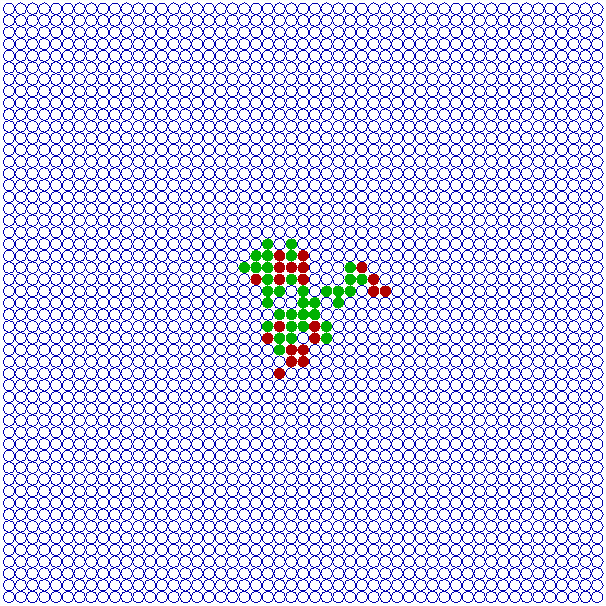
\includegraphics[width=1\textwidth, angle=0]{./fig/sir/vis/51x51agents_t50_01dt.png}
			\caption{$t = 50$}
			\label{fig:vis_51x51agents_t50_01dt}
		\end{subfigure}
    	
    	&
  
		\begin{subfigure}[b]{0.4\textwidth}
			\centering
			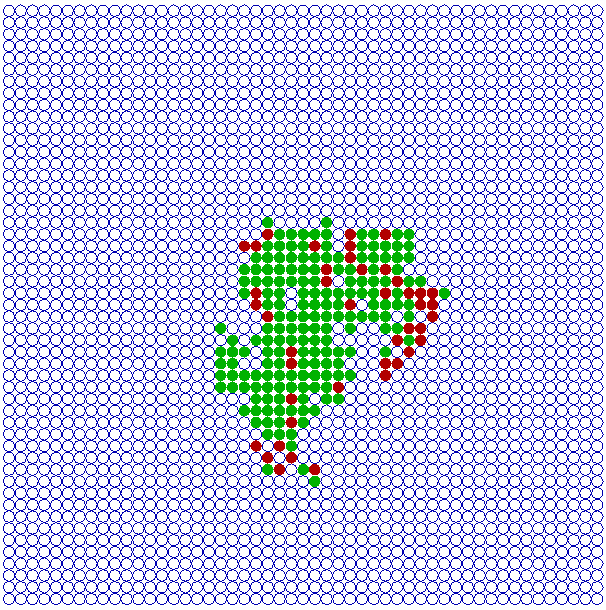
\includegraphics[width=1\textwidth, angle=0]{./fig/sir/vis/51x51agents_t100_01dt.png}
			\caption{$t = 100$}
			\label{fig:vis_51x51agents_t100_01dt}
		\end{subfigure}
	\end{tabular}
	
	\caption{Simulating the agent-based SIR model on a 51x51 2D grid with Moore neighbourhood, a single infected agent at the center, contact rate $\beta = \frac{1}{5}$, infection probability $\gamma = 0.05$ and illness duration $\delta = 15$ . Simulation run until $t = 100$ with fixed $\Delta t = 0.1$. The susceptible agents are rendered as blue hollow circles for better contrast.}
	\label{fig:vis_sir}
\end{center}
\end{figure}

\subsection{Experiment Design}
In this case study we compare the performance of the following implementations under varying numbers of CPU cores and agent numbers:

\begin{enumerate}
	\item Sequential - This is the original implementation we also discuss in TODO: cite my own PFE paper. In it the discrete 2D grid is shared amongst all agents using the State Monad. Agents are run sequentially after another thus ensuring exclusive read/write access to it. Because we are neither running in the STM or IO Monad there is no way we can run this implementation concurrently.
	\item STM - This is the same implementation like the State Monad but instead of sharing the discrete 2D grid in a State Monad, agents run in the STM Monad and have access to the discrete 2D grid through a transactional variable \textit{TVar}. This means that the reads and writes of the discrete 2D grid are exactly the same but happen always through the \textit{TVar}. Also each agent is run within its own thread, thus enabling true concurrency when the simulation is actually run on multiple cores (which can be configured by the Haskell Runtime System).
	\item Lock-Based - This is exactly the same implementation like the STM Monad but instead of running in STM, the agents now run in IO. They share the discrete 2D grid using an \textit{IORef} and have access to an \textit{MVar} to synchronise access to the it. Also each agent is run within its own thread.
	\item RePast - To have an idea where the functional implementation is performance-wise compared to the established object-oriented methods, we implemented a Java version of the SIR model using RePast with the State-Chart feature. This implementation cannot run on multiple cores concurrently but gives a good estimate of the single core performance of imperative approaches. Also there exists a RePast High Performance Computing library for implementing large-scale distributed simulations in C++ - we leave this for further research as an implementation and comparison is out of scope of this paper.
\end{enumerate}

Each experiment was run until $t = 100$ and stepped using $\Delta t = 0.1$ except in RePast for which we don't have access to the underlying implementation of the state-chart and left it as it is. For each experiment we conducted 8 runs on our machine (see Table \ref{tab:machine_specs}) under no additional work-load and report the average. Further, we checked the visual outputs and the dynamics and they look qualitatively the same to the reference implementation of the State Monad TODO: cite my own PFE paper. In the experiments we varied the number of agents (grid size) and the number of cores when running concurrently - the numbers are always indicated clearly. For varying the number of cores we compiled the executable using \textit{stack} and the \textit{threaded} option and executed it with \textit{stack} using the +RTS -Nx option where x is the number of cores between 1 and 4. 

\begin{table}
	\centering
	\begin{tabular}{ c || c }
		OS & Fedora 28 64-bit \\ \hline
		RAM & 16 GByte \\ \hline
		CPU & Intel Core i5-4670K @ 3.40GHz x 4 \\ \hline
		HD & 250Gbyte SSD \\ \hline
		Haskell & GHC 8.2.2 \\ \hline
		Java & OpenJDK 1.8.0 \\ \hline
		RePast & 2.5.0.a
	\end{tabular}
	
	\caption{Machine and Software Specs for all experiments}
	\label{tab:machine_specs}
\end{table}

\subsection{Constant Grid Size, Varying Cores}
In this experiment we held the grid size constant to 51 x 51 (2,601 agents) and varied the cores where possible. The results are reported in Table \ref{tab:constgrid_varyingcores}.

\begin{table}
	\centering
  	\begin{tabular}{ c || c | c  }
                    & Cores & Duration  \\ \hline \hline 
    	Sequential  & 1     & 100.3     \\ \hline \hline
   		STM         & 1     & 53.2      \\ \hline
   		STM         & 2     & 27.8      \\ \hline
   		STM         & 3     & 21.8      \\ \hline
   		STM         & 4     & 20.2      \\ \hline \hline
   		Lock-Based  & 1     & 60.6      \\ \hline 
   		Lock-Based  & 2     & 42.8      \\ \hline 
   		Lock-Based  & 3     & 38.6      \\ \hline 
   		Lock-Based  & 4     & 41.6      \\ \hline \hline
   		RePast      & 1     & \textbf{10.822}
  	\end{tabular}
  	
  	\caption{Experiments on constant 51x51 (2,601 agents) grid with varying number of cores.}
	\label{tab:constgrid_varyingcores}
\end{table}

%TODO: re-run the 3-core and 4-core versions of IO, i don't understand why on larger grid-sizes 4-core is faster. do 16 runs each
Comparing the performance and scaling on multiple cores of the STM and Lock-Based implementations shows that the lock-free STM implementation significantly outperforms the Lock-Based one and scales better to multiple cores. The Lock-Based implementation performs best with 3 cores and shows slightly worse performance on 4 cores as can be seen in Figure \ref{fig:core_duration_stm_io}. This is no surprise because the more cores are running at the same time, the more contention for the lock, thus the more likely synchronisation happening, resulting in more potential for reduced performance. This is not an issue in STM because no locks are taken in advance. 

Comparing the reference \textit{State} implementation shows that it is the slowest by far - even the single core STM and Lock-Based implementations outperform it by far. Also our profiling results reported about 30\% increased memory footprint for the State implementation. This shows that the State Monad is a rather slow and memory intense approach sharing data but guarantees purity and excludes any non-deterministic side-effects which is not the case in STM and IO.

What comes a bit as a surprise is that the single core RePast implementation significantly outperforms \textit{all} other implementations, even when they run on multiple cores and even with RePast doing complex visualisation in addition (something the functional implementations don't do). We attribute this to the conceptually slower approach of functional programming. We might could have optimised parts of the code but leave this for further research.

\begin{figure}
	\centering
	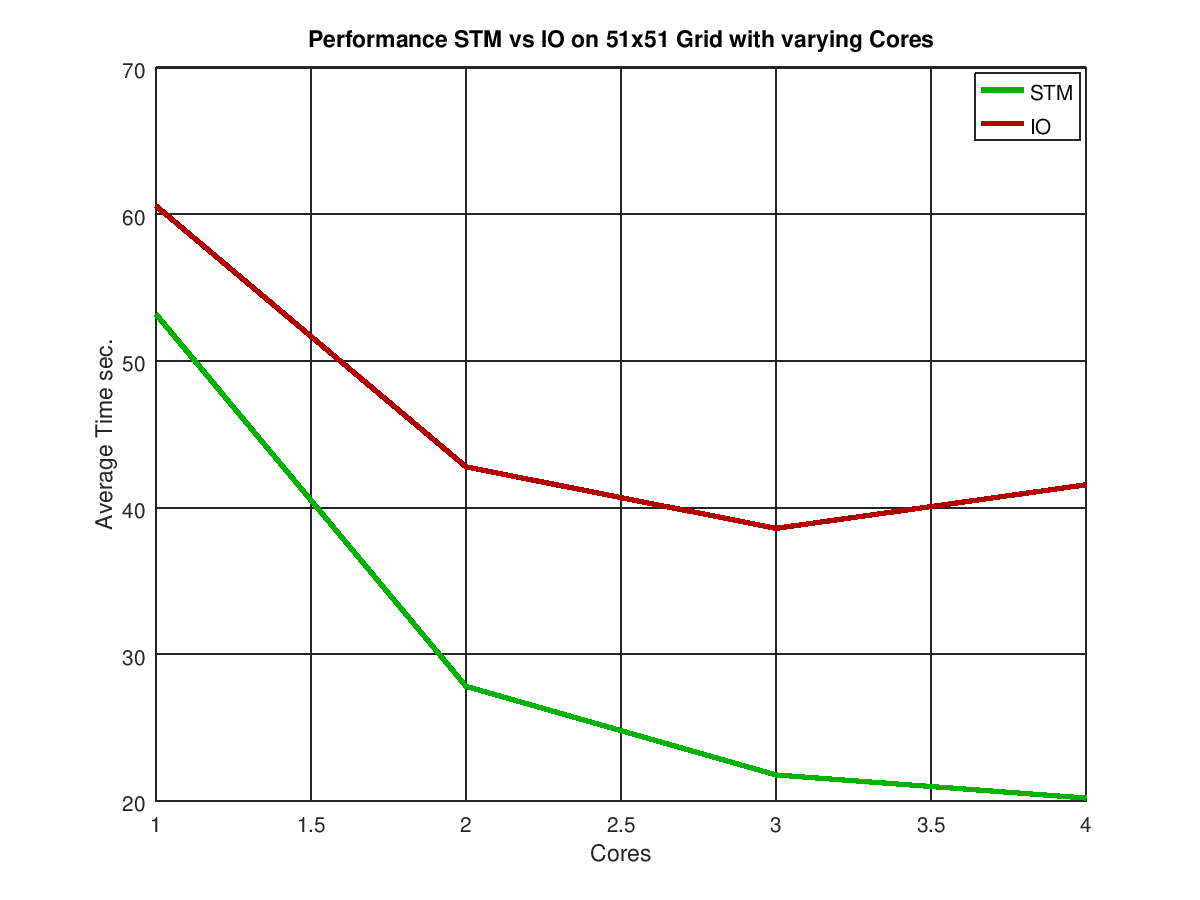
\includegraphics[width=0.6\textwidth, angle=0]{./fig/sir/core_duration_stm_io.png}
	\caption{Comparison of performance and scaling on multiple cores of STM vs. IO. Note that the Lock-Based implementation performs worse on 4 cores than on 3.}
	\label{fig:core_duration_stm_io}
\end{figure}

\subsection{Varying Grid Size, Constant Cores}
In this experiment we varied the grid size and used constantly 4 cores. Because in the previous experiment, Lock-Based performed best on 3 cores, we additionally ran Lock-Based on 3 cores as well. The results for STM are reported in Table \ref{tab:varyinggrid_constcores}. Again, note that the RePast experiments all ran on a single (1) core and were conducted to have a rough estimate where the functional approach is in comparison to the imperative.

\begin{table}
	\centering
  	\begin{tabular}{ c || c | c | c | c }
        Grid-Size          & STM              & Lock-Based (4 cores) & Lock-Based (3 cores) & RePast (1 core) \\ \hline \hline 
   		51 x 51 (2,601)    & 20.2             & 41.9                 & 38.6                 & \textbf{10.8}\\ \hline
   		101 x 101 (1,0201) & \textbf{74.5}    & 170.5                & 171.6                & 107.40 \\ \hline
   		151 x 151 (22,801) & \textbf{168.5}   & 376.9 (0)              & 404.1 (0)              & 464.017  (0) \\ \hline
   		201 x 201 (40,401) & \textbf{302.4}   & 672.0 (0)              & 720.6 (0)              & 1,227.68 (0)  \\ \hline
   		251 x 251 (63,001) & \textbf{495.7} (0) & 1,027.3 (0)            & 1,117.2 (0)            &3 ,283.63 (0)
  	\end{tabular}

  	\caption{Performance on varying grid sizes.}
	\label{tab:varyinggrid_constcores}
\end{table}

We plotted the results in Figure \ref{fig:stm_io_repast_varyinggrid_performance}. It is clear that the lock-free STM implementation outperforms the lock-based Lock-Based implementation by a substantial factor. Surprisingly, the Lock-Based implementation on 4 core scales just slightly better with increasing agents number than on 3 cores, something we wouldn't have anticipated based on the results seen in Table \ref{tab:constgrid_varyingcores}. Also  while on a 51x51 grid the single (1) core Java RePast version outperforms the 4 core Haskell STM version by a factor of 2. The figure is inverted on a 251x251 grid where the 4 core Haskell STM version outperforms the single core Java Repast version by a factor of 6. This might not be entirely surprising because we compare single (1) core against multi-core performance - still the scaling is indeed impressive and we would never have anticipated an increase of factor 6.

\begin{figure}
\begin{center}
	\begin{tabular}{c c}
		\begin{subfigure}[b]{0.5\textwidth}
			\centering
			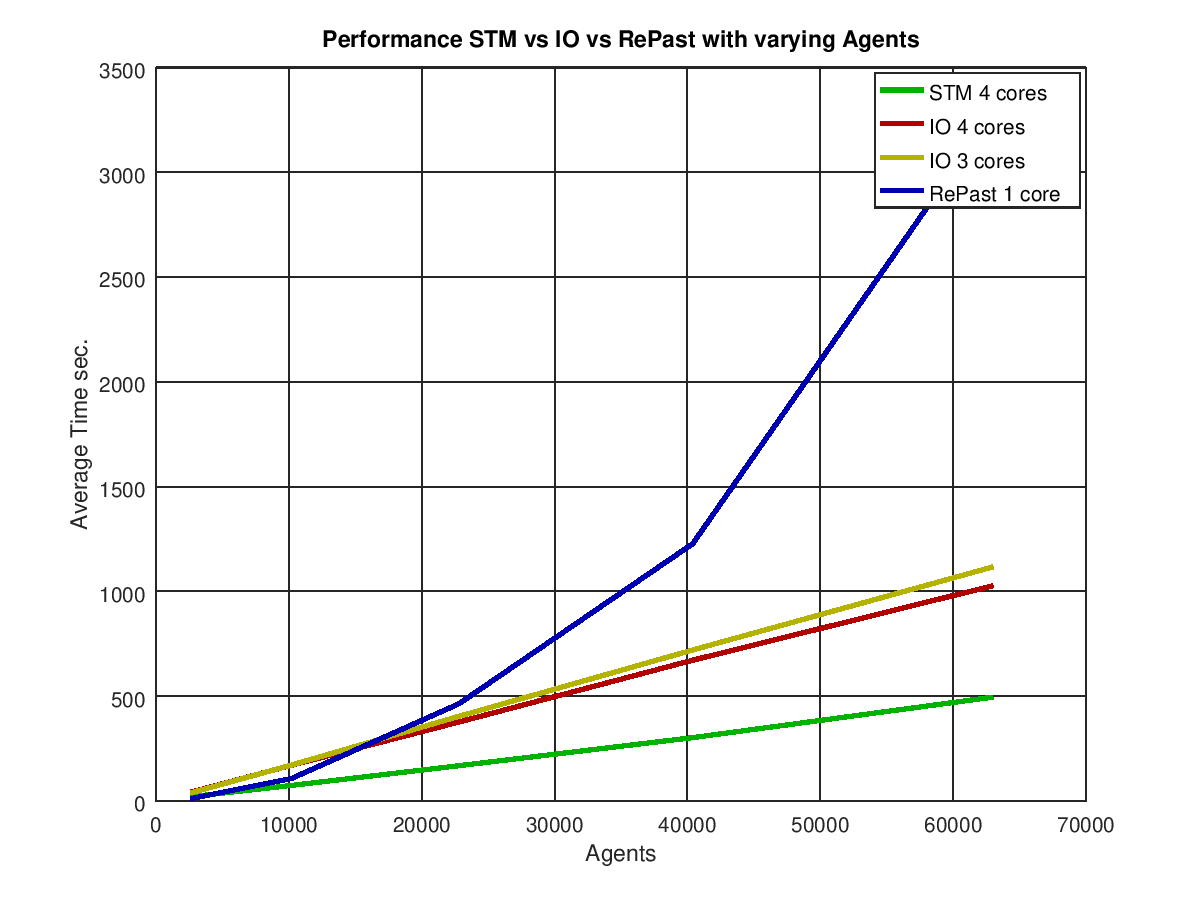
\includegraphics[width=1\textwidth, angle=0]{./fig/sir/stm_io_repast_varyinggrid_performance.png}
			\caption{Normal Scale}
		\end{subfigure}
    	&
		\begin{subfigure}[b]{0.5\textwidth}
			\centering
			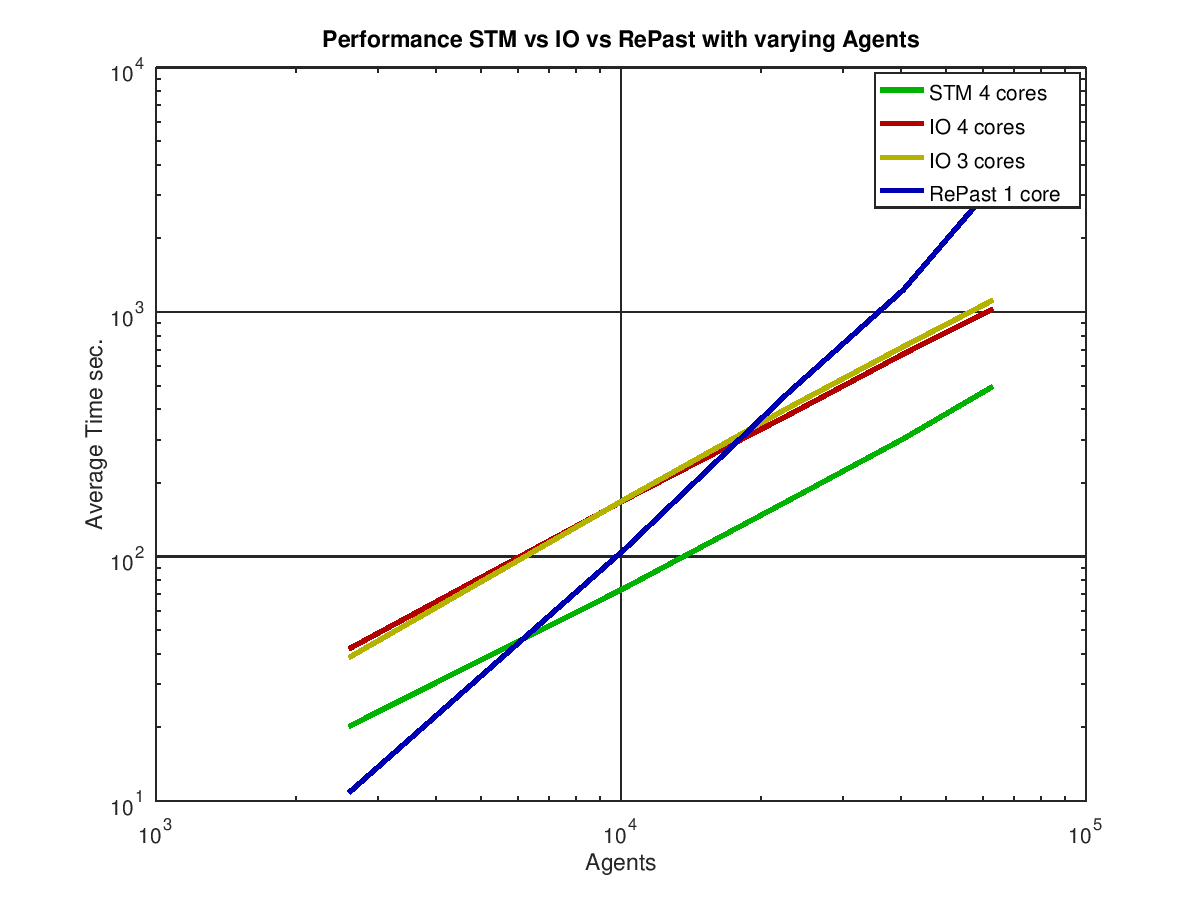
\includegraphics[width=1\textwidth, angle=0]{./fig/sir/stm_io_repast_varyinggrid_performance_loglog.png}
			\caption{Logarithmic scale on both axes}
		\end{subfigure}
    \end{tabular}
	\caption{Comparison of STM (Table \ref{tab:varyinggrid_constcores_stm}), Lock-Based (Table \ref{tab:varyinggrid_constcores4_IO}, Table 					\ref{tab:varyinggrid_constcores3_IO}) and RePast (single core) (Table \ref{tab:varyinggrid_constcores_repast}) performance. TODO: re-create the figure when all experiments had 8 runs.}
	\label{fig:stm_io_repast_varyinggrid_performance}
\end{center}
\end{figure}

\subsection{Retries}
Of very much interest when using STM is the retry-ratio, which obviously depends highly on the read-write patterns of the respective model. We used the stm-stats library to record statistics of commits, retries and the ratio. In these experiments we only averaged over 4 runs because they all arrived at a ratio of 0.0. The results are reported in Table \ref{tab:retries_stm}.

\begin{table}
	\centering
  	\begin{tabular}{ c || c | c | c }
        Grid-Size 		   & Commits    & Retries  & Ratio \\ \hline \hline 
   		51 x 51 (2,601)    & 2,601,000  & 1306.5   & 0.0 \\ \hline
   		101 x 101 (10,201) & 10,201,000 & 3712.5   & 0.0 \\ \hline
   		151 x 151 (22,801) & 22,801,000 & 8189.5   & 0.0 \\ \hline
   		201 x 201 (40,401) & 40,401,000 & 13285 (0.0) & 0.0 \\ \hline 
   		251 x 251 (63,001) & 63,001,000 & 21217 (0.0) & 0.0
  	\end{tabular}
  	
  	\caption{Retries Ratio of STM Monad experiments on varying grid sizes on 4 cores.}
	\label{tab:retries_stm}
\end{table}

Independent of the number of agents we always have a retry-ratio of 0.0. This indicates that this model is \textit{very} well suited to STM, which is also directly reflected in the substantial better performance over the Lock-Based implementation. Obviously this ratio stems from the fact, that in our implementation we have \textit{very} few writes (only when an agent changes e.g. from Susceptible to Infected or from Infected to Recovered) and mostly reads. Also we conducted runs on lower number of cores which resulted in fewer retries, which was what we expected.

\subsection{Going Large-Scale}
To test how far we can scale up the number of cores in both the \textit{Lock-Based} and \textit{TArray} cases, we ran the two experiments (51x51 and 251x251) on Amazon S2 instances with increasing number of cores starting with 16 until we ran into decreasing returns. The results are reported in Table \ref{tab:varying_cores_amazon} and can be seen in Figure \ref{fig:varying_cores_amazon}.

\begin{table}
	\centering
  	\begin{tabular}{ c || c | c | c }
                   & Cores & 51x51   & 251x251 \\ \hline \hline 
    	Lock-Based & 16    & TODO    & TODO    \\ \hline
    	Lock-Based & 32    & TODO    & TODO    \\ \hline
   		
   		STM        & 16    & TODO    & TODO    \\ \hline
   		STM        & 32    & TODO    & TODO    \\ \hline
   	\end{tabular}
  	
  	\caption{Performance on varying cores in Amazon S2 Cloud.}
	\label{tab:varying_cores_amazon}
\end{table}

\subsection{Discussion}
Reflecting of the performance data leads to the following insights:
\begin{enumerate}
	%\item On a single core, no transaction retries should happen, the results support that assumption.
	\item Running in STM and sharing state using a transactional variable is much more time- and memory-efficient than running in the State Monad but potentially sacrifices determinism: repeated runs might not lead to same dynamics despite same initial conditions.
	\item Running STM on multiple cores concurrently \textit{does} lead to a significant performance improvement \textit{for that model}.
	\item STM outperforms the Lock-Based implementation substantially and scales much better to multiple cores.
	\item STM on single (1) core is still about twice as slow than an object-oriented Java RePast implementation on a single (1) core.
	\item STM on multiple cores dramatically outperforms the single (1) core object-oriented Java RePast implementation on a single (1) core on instances with large agent numbers and scales much better to increasing number of agents.
\end{enumerate}

\section{Case Study 2: SugarScape} %(Second Encounter)
\label{sec:cs_sugarscape}

One of the first models in Agent-Based Simulation was the seminal Sugarscape model developed by Epstein and Axtell in 1996 \cite{epstein_growing_1996}. Their aim was to \textit{grow} an artificial society by simulation and connect observations in their simulation to phenomenon observed in real-world societies. In this model a population of agents move around in a discrete 2D environment where sugar grows and interact with each other and the environment in many different ways. The main features of this model are (amongst others): searching, harvesting and consuming of resources, wealth and age distributions, population dynamics under sexual reproduction, cultural processes and transmission, combat and assimilation, bilateral decentralized trading (bartering) between agents with endogenous demand and supply, disease processes transmission and immunology.

We implemented the \textit{Carrying Capacity} (p. 30) section of Chapter II of the book \cite{epstein_growing_1996}. There, in each step agents search (move) to the cell with the highest sugar they see within their vision, harvest all of it from the environment and consume sugar because of their metabolism. Sugar regrows in the environment over time. Only one agent can occupy a cell at a time. Agents don't age and cannot die from age. If agents run out of sugar due to their metabolism, they die from starvation and are removed from the simulation. The authors report that the initial number of agents quickly drops and stabilises around a level depending on the model parameters. This is in accordance with our results as we show in Figure \ref{fig:vis_sugarscape} and guarantees that we don't run out of agents. The model parameters are as follows:

\begin{itemize}
	\item Sugar Endowment: each agent has an initial sugar endowment randomly uniform distributed between 5 and 25 units.
	\item Sugar Metabolism: each agent has a sugar metabolism randomly uniform distributed between 1 and 5.
	\item Agent Vision: each agent has a vision randomly uniform distributed between 1 and 6, same for each of the 4 directions (N, W, S, E). 
	\item Sugar Growback: sugar grows back by 1.0 unit per step until the maximum capacity of a cell is reached.
	\item Agent Number: initially 500 agents.
	\item Environment Size: 50 x 50 cells with toroid boundaries which wrap around in both x and y dimension.
\end{itemize}

\begin{figure}
\begin{center}
	\begin{tabular}{c c}
		\begin{subfigure}[b]{0.4\textwidth}
			\centering
			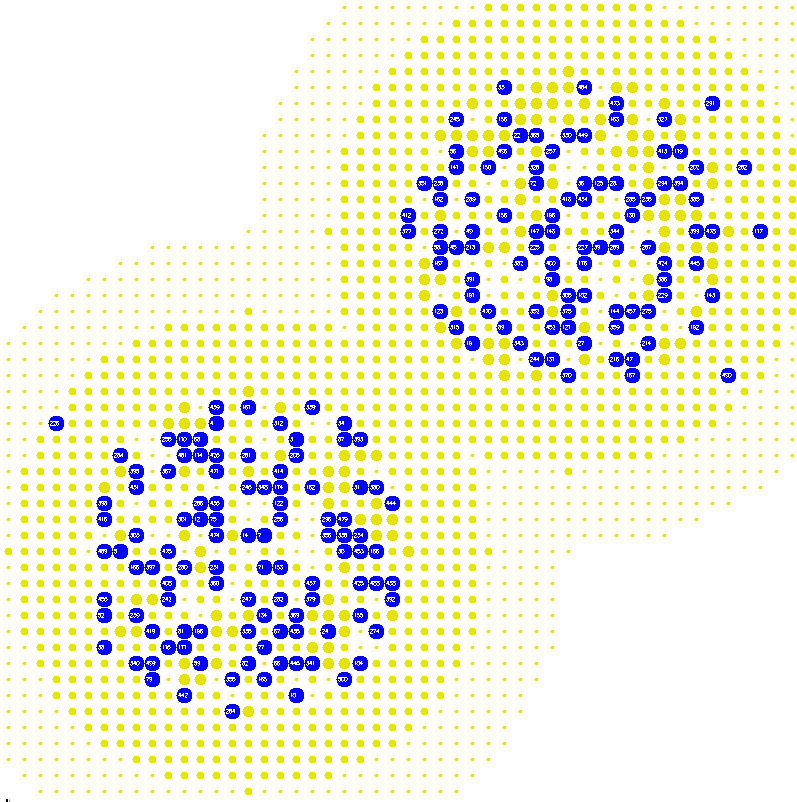
\includegraphics[width=1\textwidth, angle=0]{./fig/sugarscape/vis/sugarscape_t60_environment.png}
			\caption{Visualisation of the Sugarscape at $t = 50$}
			\label{fig:vis_sugarscape_t50_environment}
		\end{subfigure}
    	
    	&
  
		\begin{subfigure}[b]{0.6\textwidth}
			\centering
			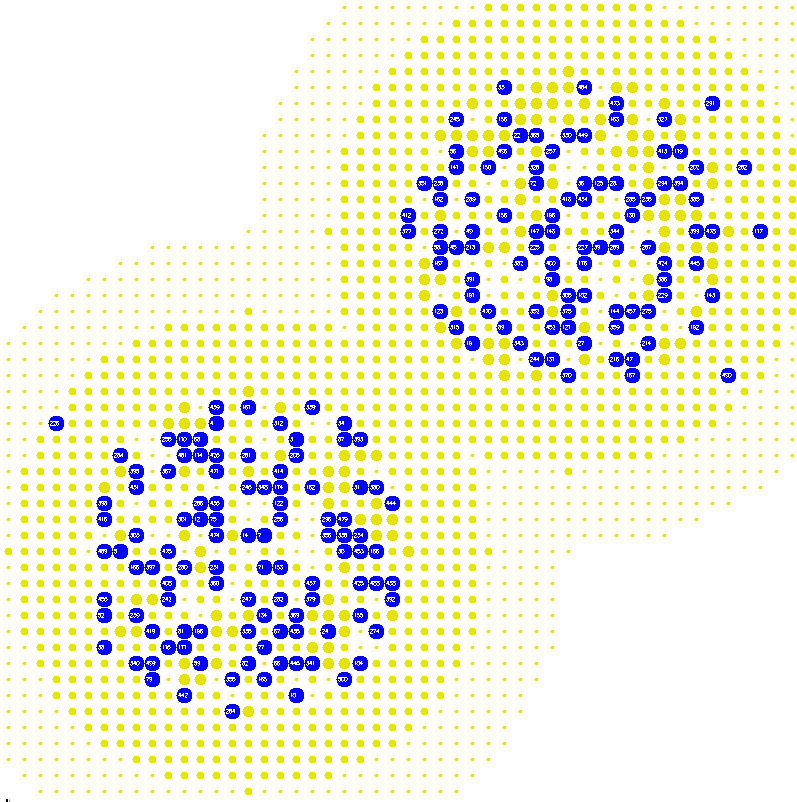
\includegraphics[width=1\textwidth, angle=0]{./fig/sugarscape/vis/sugarscape_t60_dynamics.png}
			\caption{Dynamics population size over 50 steps}
			\label{fig:vis_sugarscape_t50_dynamics}
		\end{subfigure}
	\end{tabular}
	
	\caption{Visualisation of our SugarScape implementation and dynamics of the population size over 50 steps. The white numbers in the blue agent circles are the agents unique ids.}
	\label{fig:vis_sugarscape}
\end{center}
\end{figure}

\subsection{Experiment Design}
We compare three different implementations

\begin{enumerate}
	\item Sequential - All agents are run after another (including the environment) and the environment is shared amongst the agents using the State Monad.
	\item Lock-Based - All agents are run concurrently and the environment is shared using an \textit{IORef} amongst the agents which acquire and release a lock when accessing it.
	\item STM TVar - All agents are run concurrently and the environment is shared using a \textit{TVar} amongst the agents.
	\item STM TArray - All agents are run concurrently and the environment is shared using a \textit{TArray} amongst the agents. 
\end{enumerate}

The model specification requires to shuffle agents before every step (Footnote 12 on page 26). In the \textit{Sequential} approach we do this explicitly but in both STM approaches this happens automatically due to race-conditions in concurrency thus we arrive at an effectively shuffled processing of agents: we can assume that the order of the agents is \textit{effectively} random in every step. The important difference between the two approaches is that in the State approach we have full control over this randomness but in the STM not - also this means that repeated runs with the same initial conditions might lead to slightly different results.
Note that in the concurrent implementations we could have two options for running the environment: either running it asynchronously as a concurrent agent at the same time with the population agents or synchronously after all agents have run. We must be careful though as running the environment as a concurrent agent can be seen as conceptually wrong because the time when the regrowth of the sugar happens is now completely random. It could happen in the very first transaction or in the very last, different in each step, which can be seen as a violation of the model specifications (TODO: reference the book where it shows that environment grows after / before all agents).

We follow \cite{lysenko_framework_2008} and measure the average updates per second of the simulation over 60 seconds.

For each experiment we conducted 8 runs on our machine (see Table \ref{tab:machine_specs}) under no additional work-load and report the average. In the experiments we varied the number of cores when running concurrently - the numbers are always indicated clearly. For varying the number of cores we compiled the executable using \textit{stack} and the \textit{threaded} option and executed it with \textit{stack} using the \textit{+RTS -Nx} option where x is the number of cores between 1 and 4.

Note that we omit the graphical rendering in the functional approach because it is a serious bottleneck taking up substantial amount of the simulation time. Although visual output is crucial in ABS, it is not what we are interested here thus we completely omit it and only output the number of agents in the simulation at each step piped into a file, thus omitting slow output to the console. Note that we need to produce \textit{some} output because of Haskells laziness - if we wouldn't output anything from the simulation then the expressions would actually never be fully evaluated thus resulting in ridiculous high number of steps per second but which obviously don't really reflect the true computations done.

\subsection{Constant Agent Size}
In this first approach we compare the performance of all implementations on varying numbers of cores. The results are reported in Table \ref{tab:varying_cores} and can be seen in Figure \ref{fig:varying_cores}. 

\begin{table}
	\centering
  	\begin{tabular}{ c || c | c | c }
                   & Cores & Steps & Retries  \\ \hline \hline 
    	Sequential & 1     & 39.4  & N/A      \\ \hline \hline   

    	Lock-Based & 1     & 43.0  & N/A       \\ \hline
    	Lock-Based & 2     & 51.8  & N/A       \\ \hline
    	Lock-Based & 3     & 57.4  & N/A       \\ \hline
    	Lock-Based & 4     & 58.1  & N/A       \\ \hline \hline   
   		
   		STM TVar   & 1     & 47.3  & 0.0       \\ \hline
   		STM TVar   & 2     & 53.5  & 1.1       \\ \hline
   		STM TVar   & 3     & 57.1  & 2.2 	   \\ \hline
   		STM TVar   & 4     & 53.0  & 3.2	   \\ \hline \hline   
   		
   		STM TArray & 1     & 45.4  & 0.0 	   \\ \hline
   		STM TArray & 2     & 65.3  & 0.02      \\ \hline
   		STM TArray & 3     & 75.7  & 0.04      \\ \hline
   		STM TArray & 4     & 84.4  & 0.05	   \\ \hline \hline   
   	\end{tabular}
  	
  	\caption{Steps per second and retries on 50x50 grid and 500 initial agents on varying cores.}
	\label{tab:varying_cores}
\end{table}

\begin{figure}
	\centering
	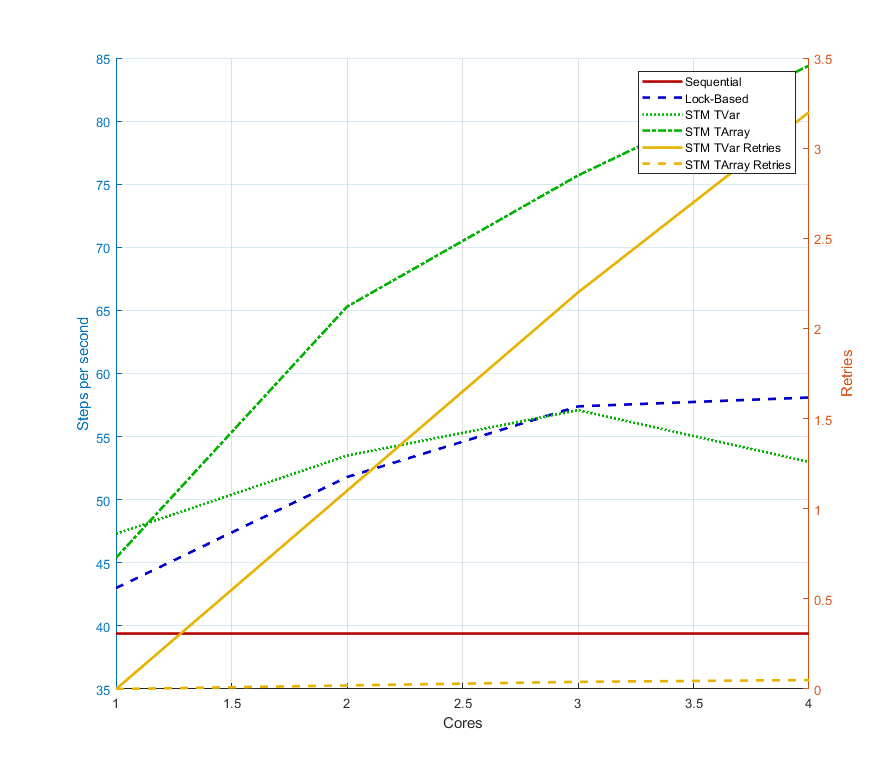
\includegraphics[width=0.7\textwidth, angle=0]{./fig/sugarscape/varying_cores.png}
	\caption{Steps per second and retries on 50x50 grid and 500 initial agents on varying cores.}
	\label{fig:varying_cores}
\end{figure}

As expected, the \textit{Sequential} implementation is the slowest, followed by the \textit{Lock-Based} and \textit{TVar} approach whereas \textit{TArray} is the best performing one.

We clearly see that using \textit{TVar} to share the environment is a very inefficient choice: \textit{every} write to a cell leads to a retry independent whether the reading agent read that changed cell or not because the data-structure can not distinguish between individual cells. By using a \textit{TArray} we can avoid the situation where a write to a cell in a far distant location of the environment will lead to a retry of an agent which never even touched that cell. Also the \textit{TArray} seems to scale up by 10 steps per second for every core added, it would be interesting to see how far this could go as we seem not to hit a limit with 4 cores yet. We leave this for further research.

The inefficiency of \textit{TVar} is also reflected in the nearly similar performance of the \textit{Lock-Based} implementation which even outperforms it on 4 cores. This is due to very similar approaches because both operate on the whole environment instead of only the cells as \textit{TArray} does. This seems to be a bottleneck in \textit{TVar} reaching the best performance on 3 cores which then drops on 4 cores which the \textit{Lock-Based} approach seems to be able to avoid but reducing its returns on increased number of cores hitting a limit there as well.

\subsection{Scaling up Agents}
So far we always kept the initial number of agents at 500, which due to the model specification, quickly drops and stabilises around 200 due to the carrying capacity of the environment as described in the book \cite{epstein_growing_1996} section \textit{Carrying Capacity} (p. 30).

We now want to see performance of our approaches under increased number of agents. For this we slightly change the implementation: always when an agent dies it spawns a new one which is inspired by the ageing and birthing feature of Chapter III in the book \cite{epstein_growing_1996}. This ensures that we keep the number of agents roughly constant (still fluctuates but doesn't drop to low levels) over the whole duration. This ensures a constant load of concurrent agents interacting with each other and demonstrates also the ability to terminate and fork threads dynamically during the simulation.

Except for the \textit{Sequential} approach we ran all experiments with 4 (3) cores. We looked into the performance of 500, 1,000, 1,500, 2,000 and 2,500 (maximum possible capacity of the 50x50 environment). The results are reported in Table \ref{tab:state_results_agentsscale_time} and can be seen in Figure \ref{fig:state_results_agentsscale_time}.

\begin{table}
	\centering
  	\begin{tabular}{ c || c | c | c | c | c }
        Agents  & Sequential & Lock-Based & TVar (3 cores) & TVar (4 cores) & TArray  \\ \hline \hline 
    	500     & 14.4       & 20.2		  &	20.1           & 18.5       	& 71.9    \\ \hline
   		1,000   & 6.8        & 10.8 	  & 10.4           & 9.5       	    & 54.8    \\ \hline
   		1,500   & 4.7        & 8.1 		  & 7.9            & 7.3			& 44.1    \\ \hline
   		2,000   & 4.4        & 7.6 		  & 7.4            & 6.7    		& 37.0    \\ \hline 
   		2,500   & 5.3        & 5.4 		  & 9.2            & 8.9			& 33.3
   	\end{tabular}
  	
  	\caption{Steps per second on 50x50 grid and varying number of agents with 4 (and 3) cores except Sequential (1 core).}
	\label{tab:state_results_agentsscale_time}
\end{table}

\begin{figure}
	\centering
	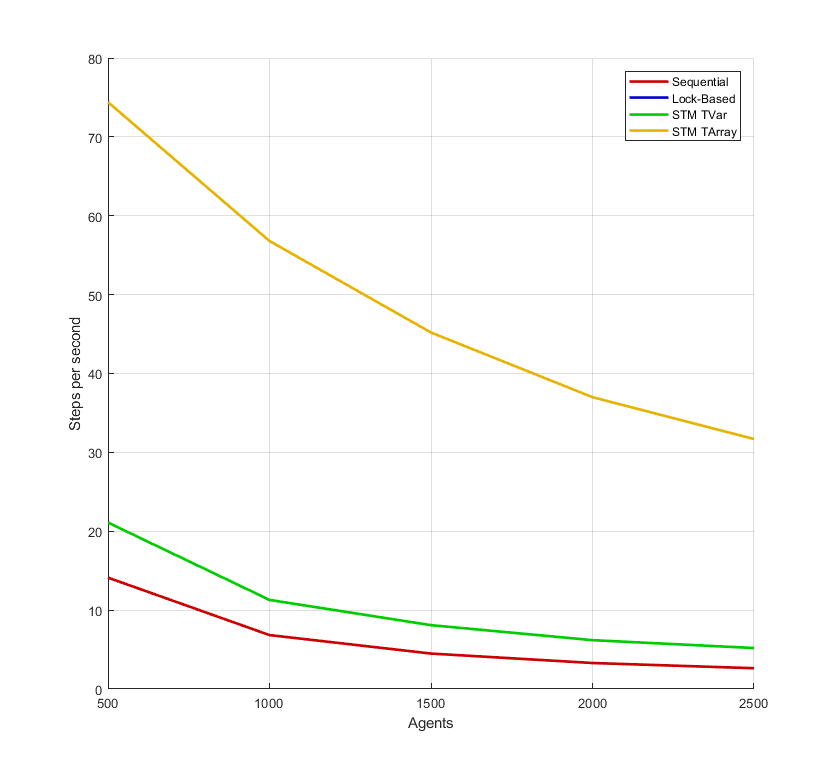
\includegraphics[width=0.6\textwidth, angle=0]{./fig/sugarscape/varying_agents.png}
	\caption{Steps per second on 50x50 grid and varying number of agents with 4 (and 3) cores except Sequential (1 core).}
	\label{fig:state_results_agentsscale_time}
\end{figure}

As expected, the \textit{TArray} implementation outperforms all others substantially. Also as expected, the \textit{TVar} implementation on 3 cores is faster than on 4 cores as well when scaling up to more agents. The \textit{Lock-Based} approach performs about the same as the \textit{TVar} on 3 cores because of the very similar approaches: both access the \textit{whole} environment. Still the \textit{TVar} approach uses one core less to arrive at the same performance, thus strictly speaking outperforming the \textit{Lock-Based} implementation.

What seems to be very surprising is that in the \textit{Sequential} and \textit{TVar} cases the performance with 2,500 agents is \textit{better} than the one with 2,000 agents. The reason for this is that in the case of 2,500 agents, when an agent tries to move it can't move anywhere because all cells are already occupied. In this case the agent won't rank the cells in order of their pay-off (max sugar) to move to but just stays where it is.  Due to Haskells laziness the agents actually never look at the content of the cells in this case but only the number which means that the cells themselves are never evaluated which further increases performance. This leads to the better performance in case of \textit{Sequential} and \textit{TVar} because both exploit laziness.
In the case of the \textit{Lock-Based} approach we still arrive at a lower performance because the limiting factor are the unconditional locks. In the case of the \textit{TArray} approach we also arrive at a lower performance because we perform STM reads on the neighbouring cells which are not subject to lazy evaluation.

We also measured the average retries both for \textit{TVar} and \textit{TArray} under 2,500 agents where the \textit{TArray} approach shows best scaling performance with 0.01 retries whereas \textit{TVar} averages at 3.28 retries. Again this can be attributed to the better transactional data-structure which reduces retry-ratio substantially to near-zero levels.

\subsection{Going Large-Scale}
To test how far we can scale up the number of cores in both the \textit{Lock-Based} and \textit{TArray} cases, we ran the two experiments (carrying capacity and rebirthing) on Amazon S2 instances with increasing number of cores starting with 16 until we ran into decreasing returns. The results are reported in Table \ref{tab:sug_varying_cores_amazon}.

\begin{table}
	\centering
  	\begin{tabular}{ c || c | c | c }
                   & Cores & Carrying Capacity & Rebirthing \\ \hline \hline 
    	Lock-Based & 16    & 53.9              & 4.4        \\ \hline
    	Lock-Based & 32    & 44.2              & 3.6        \\ \hline \hline 
   		
   		STM TArray & 16    & 116.8             & 39.5       \\ \hline
   		STM TArray & 32    & 109.8             & 31.3       \\ \hline
   	\end{tabular}
  	
  	\caption{Steps per second on varying cores on Amazon S2 Services.}
	\label{tab:sug_varying_cores_amazon}
\end{table}

As expected, the \textit{Lock-Based} approach doesn't scale up to many cores because each additional core brings more contention to the lock, resulting in even more decreased performance. This is particularly obvious in the rebirthing experiment because of the much larger number of concurrent agents. The \textit{TArray} approach returns better performance on 16 cores but fails to scale further up to 32 where the performance drops below the one with 16 cores. At this point we are running into Amdahls law and become dominated by the sequential part of the program which is the main lock-step mechanism and environment process.

\subsection{Comparison with other approaches}
The paper \cite{lysenko_framework_2008} reports a performance of 17 steps in RePast, 18 steps in MASON (both non-parallel) and 2000 steps per second on a GPU on a 128x128 grid. Although our \textit{Sequential} implementation which runs non-parallel as well outperforms the RePast and MASON implementations one must be very well aware that these results were generated in 2008, on 10 year older hardware - the performance might have caught up by now and even outperform our functional \textit{Sequential} approach. 

Indeed, when we run the SugarScape example of RePast with the same model parameters as ours on the same machine (see Table \ref{tab:machine_specs}) we arrive at roughly 450 steps per second - a factor of more than 5 faster than even our STM \textit{TArray} implementation on 4 cores. This might seem quite shocking, even more so because RePast also performs visual output, rendering the SugarScape in every step. When scaling up the agents to 2,500 the RePast version arrives around roughly 95 steps per second which is still faster by a factor of 3 than our 4 core \textit{TArray} implementation. We attribute this substantial performance difference to  the inherent deeper complexity of the model where it seems that imperative implementations seem to have an advantage. Still our research is just a first step and might result in future work increasing performance.

The very high performance on the GPU does not concern us here as it follows a very different approach than we do here. Our focus is on speeding up implementations on the CPU as directly as possible without locking overhead. When following a GPU approach one needs to map the model to the GPU which is a delicate and non-trivial approach. With our approach we show that speed-up with concurrency is very possible without the low-level locking details or the need to map to GPU. Also some feature as bilateral trading between agents where a pair of agents need to come to a conclusion over multiple synchronous steps is difficult or even impossible to implement on a GPU whereas this is easily possible using STM on a CPU as well.

Note that we kept the grid-size constant because we implemented the environment as a single agent which works sequentially on the cells to regrow the sugar. Obviously this doesn't really scale up on parallel hardware and experiments which we haven't included here show that the performance goes down dramatically when we increase the environment to 128x128 with same number of agents which is the result of Amdahl's law where the environment becomes the limiting factor of the simulation. Depending on the underlying data-structure used for the environment we have two options to solve this problem. In the case of the \textit{Sequential} and \textit{TVar} implementation we build on an indexed array which we can be updated in parallel using the existing data-parallel support in Haskell. In the case of the \textit{TArray} approach we have no option but to run the update of every cell within its own thread. We leave both for further research as it is out of scope of this paper.

\subsection{Discussion}
Reflecting of the performance data leads to the following insights:
\begin{itemize}	
	\item Selecting the right transactional data-structure is very model-specific and can lead to dramatically different performance results. In this case the \textit{TArray} performed best due to many writes, in the SIR case-study a \textit{TVar} showed good enough results due to the very low number of writes.
	\item A \textit{TArray} might come with an overhead, performing worse on low number of cores than a \textit{TVar} approach but has the benefit of quickly scaling up to multiple cores.
	\item When not carefully selecting the right transactional data-structure which supports fine-grained concurrency a lock-based implementation might perform as well or even outperform the STM approach as can be seen when using the \textit{TVar}.
	\item Depending on the transactional data-structure scaling up to multiple cores hits a limit earlier or later. In the case of the \textit{TVar} the best performance is reached with 3 cores. With the \textit{TArray} we didn't reach this limit yet with 4 cores - we leave this for further research as it might be well beyond tens of cores.
	\item A well implemented STM approach with a  carefully selected transactional data-structure consistently outperforms the lock-based approach and scales up to multiple cores considerably better.
	\item Generalise the insight of 2,500 better than 2,000
	\item Unfortunately for this model the performance is nowhere comparable to imperative approaches which we attribute to the inherent deeper complexity of the model where it seems that imperative implementations seem to have an advantage.
\end{itemize}

\chapter{Conclusions}
\label{chap:concl}

\section{Being Realistic}
It is of most importance to stress that we don't condemn the current state-of-the-art approach of object-oriented specification and implementation to ABS. The strength of object-oriented programming is surely that it can be seen as \textit{programming as modelling} and thus will be always an attractive approach to ABS. Also we are realists and know that there are more points to consider when selecting a set of methods for developing software for an ABS than robustness, verification and validation. Almost always the popularity of an existing language and which languages the implementer knows is the driving force behind which methods and languages to choose. This means that ABS will continue to be implemented in object-oriented programming languages and many perfectly well functioning models will be created by it in the future. Although they all suffer from the same issues mentioned in the introduction this doesn't matter as they are not of central importance to most of them.
Nonetheless we think our work is still essential and necessary as it may start a slow paradigm-shift and opens up the minds of the ABS community to a more functional and formal way of approaching and implementing agent-based models and simulations and recognizing the benefits one gets automatically from it by doing so.

\section{What we are not doing}
Because of this highly interdisciplinary topic we explicitly mention what we do not want to undertake in this PhD.
First we don't want to develop another language for formal agent-specification which needs to be compiled or used in some fancy tool - we want to put it directly into Haskell, building on the existing facilities.
Second, we are not developing a new economic theory about decentralized bilateral bartering, we take the existing theory and existing agent-based models and apply our methods to them.
Third, we don't want to use fancy statistics and number juggling for comparing validating and verifying models: we want structural comparison (category-theory).
Fourth, we do NOT want to do a direct comparison of object-orientation vs. functional in ABS, as we would get lost in an infinite amount of low-level technical details. We look at the benefits / drawbacks more on a conceptual level, applied to ABS.

\section{Further Research}
\label{sec:further_research}
We see this paper as an intermediary and necessary step towards dependent types for which we first needed to understand the potential and limitations of a non-dependently typed pure functional approach in Haskell. Dependent types are extremely promising in functional programming as they allow us to express stronger guarantees about the correctness of programs and go as far as allowing to formulate programs and types as constructive proofs which must be total by definition \cite{thompson_type_1991, mckinna_why_2006, altenkirch_pi_2010}.

So far no research using dependent types in agent-based simulation exists at all. In our next paper we want to explore this for the first time and ask more specifically how we can add dependent types to our pure functional approach, which conceptual implications this has for ABS and what we gain from doing so. We plan on using Idris \cite{brady_idris_2013} as the language of choice as it is very close to Haskell with focus on real-world application and running programs as opposed to other languages with dependent types e.g. Agda and Coq which serve primarily as proof assistants.

We hypothesize that dependent types could help ruling out even more classes of bugs at compile time and encode invariants and model specifications on the type level, which implies that we don't need to test them using e.g. property-testing with QuickCheck. This would allow the ABS community to reason about a model directly in code. We think that a promising approach is to follow the work of \cite{brady_correct-by-construction_2010, brady_idris_2011, brady_programming_2013, fowler_dependent_2014, brady_state_2016} in which the authors utilize GADTs to implement an indexed monad which allows to implementation correct-by-construction software.

\begin{itemize}
% NOTE: ran out of space
%	\item Accessing the environment in section \ref{sec:adding_env} involves indexed array access which is always potentially dangerous as the indices have to be checked at run-time. Using dependent types it should be possible to encode the environment dimensions into the types. In combination with suitable data types for coordinates one should be able to ensure already at compile time that access happens only within the bounds of the environment.

	\item In the SIR implementation one could make wrong state-transitions e.g. when an infected agent should recover, nothing prevents one from making the transition back to susceptible. 
	
	Using dependent types it should be possible to encode invariants and state-machines on the type level which can prevent such invalid transitions already at compile time. This would be a huge benefit for ABS because many agent-based models define their agents in terms of state-machines.
	
	\item An infected agent recovers after a given time - the transition of infected to recovered is a timed transition. Nothing prevents us from \textit{never} doing the transition at all. 
	
	With dependent types we should be able to encode the passing of time in the types and guarantee on a type level that an infected agent has to recover after a finite number of time steps.
	
	\item In more sophisticated models agents interact in more complex ways with each other e.g. through message exchange using agent IDs to identify target agents. The existence of an agent is not guaranteed and depends on the simulation time because agents can be created or terminated at any point during simulation. 
	
	Dependent types could be used to implement agent IDs as a proof that an agent with the given id exists \textit{at the current time-step}. This also implies that such a proof cannot be used in the future, which is prevented by the type system as it is not safe to assume that the agent will still exist in the next step.

	\item In our implementation, we terminate the SIR model always after a fixed number of time-steps. We can informally reason that restricting the simulation to a fixed number of time-steps is not necessary because the SIR model \textit{has to} reach a steady state after a finite number of steps. This means that at that point the dynamics won't change any more, thus one can safely terminate the simulation. Informally speaking, the reason for that is that eventually the system will run out of infected agents, which are the drivers of the dynamic. We know that all infected agents will recover after a finite number of time-steps \textit{and} that there is only a finite source for infected agents which is monotonously decreasing. 
	
	Using dependent types it might be possible to encode this in the types, resulting in a total simulation, creating a correspondence between the equilibrium of a simulation and the totality of its implementation. Of course this is only possible for models in which we know about their equilibria a priori or in which we can reason somehow that an equilibrium exists.
\end{itemize}

% Place the main text here. Please use only \section, \subsection, and \subsubsection sectioning commands to structure your text. Do NOT use lower sectioning commands, including \paragraph and \subparagraph

%For bulleted, numbered and description lists the class provides three asterisked environments to replace the standard LaTeX ones: itemize*, enumerate*, and description*. Please use these ones as the standard environment may cause issues with the paragraph numbering system.

%\begin{itemize*}
%     \item 
%     \item
%     \item
% \end{itemize*} 

% hyperlinks (to models, videos, etc.) can be included via the \href command (remember to put \usepackage{hyperref} in the preamble). Check the hyperref documentation for details

%%%%%%%%%%%%%%%%%%%%%%%%%%%%%%%%%%%%%%%%%%%%%%

% FIGURES AND TABLES

% Figures should be placed in the desired position within the text. Please follow the template below.
% Figure widths can be set using absolute dimensions (e.g., [width = 12cm]) or relative ones (e.g., [width = 0.8/textwidth]). We strongly suggest to use the latter option, as this allows automatic adaptation to different paper widths

%\begin{figure}[!t]
%\centering
%\includegraphics[width=????\textwidth]{????}
%\caption{}
%\label{fig:????}
%\end{figure}

% Tables should be placed in the desired position within the text. Please follow the template below

%\begin{table}[!t]
%	\centering
%	\begin{tabular}{????}
%	\toprule
% 	% first line
%	\midrule
%	% tale body	
%	\bottomrule			
%	\end{tabular}
%	\caption{}
%	\label{tab:????}	
%\end{table}

%%%%%%%%%%%%%%%%%%%%%%%%%%%%%%%%%%%%%%%%%%%%%%
% End of  paragraph numbering. Please leave this untouched
\endparano

%%%%%%%%%%%%%%%%%%%%%%%%%%%%%%%%%%%%%%%%%%%%%%

%%%%%%%%%%%%%%%%%%%%%%%%%%%%%%%%%%%%%%%%%%%%%%

% APPENDICES
% Put your appendices here. Please use the normal sectioning command, e.g.,
% \section{Appendix A: <title of the appendix>}
% \section{Appendix B: <title of the appendix>}
% ...

%%%%%%%%%%%%%%%%%%%%%%%%%%%%%%%%%%%%%%%%%%%%%%

% ENDNOTES. Please uncomment the line below in case of notes.
% \theendnotes

%%%%%%%%%%%%%%%%%%%%%%%%%%%%%%%%%%%%%%%%%%%%%%

% REFERENCES.
% The JASSS bibliographic style file (jasss.bst) is included in the bundle. Please use BibTeX, not BibLaTeX.
% Use natbib commands for references (\citep{}, \citet{}, etc.), not standard LaTeX ones (\cite{}).
% Remember to include the doi and url fields in your bib database. The address field should be included for books.
% Please upload the bib file (not just the bbl one) when submitting.
 
\bibliographystyle{jasss}
%\bibliography{} % Please set the right name for your bib file
\bibliography{../../../references/phdReferences.bib}

%%%%%%%%%%%%%%%%%%%%%%%%%%%%%%%%%%%%%%%%%%%%%%

\end{document}